\chapter{Парадоксы в невесомости}

\section{Гелиевый шар}

\begin{thm}{Задача}
Два космонавта, Андрей и Боря, пристёгнуты к противоположным концам космической капсулы, как показано на рисунке \ref{pic:2.1}.
В начале всё находится в покое и Андрей держит в руках большой воздушный шарик наполненный гелием.
Он толкает шарик, и тот начинает двигаться в сторону Бори.
В каком направлении начнёт двигаться сама капсула с точки зрения наблюдателя, парящего в открытом космосе вне капсулы?
Поскольку астронавты пристёгнуты к стенкам, их можно считать частью капсулы.
\end{thm}

\begin{figure}[ht!]
\centering
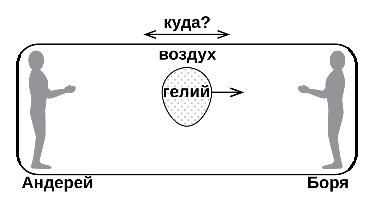
\includegraphics[scale=1]{pics/2.1}
\caption{Куда двинется капсула когда Андрей толкнёт шар?}
\label{pic:2.1}
\end{figure}
